\begin{frame}
\frametitle{Espacios Tangentes en $\R^n$}
\begin{definition}[Vectores y Espacios Tangentes en $\R^n$]\label{Definición: Espacio Tangente en Rn}
Sea $a$ un punto en $\R^n$, definiremos el \textbf{espacio tangente a $\R^n$ en el punto $a$}, denotado por $T_a(\R^n)$, como el conjunto:
  \[ \{a\} \times \R^n = \{(a,v): v \in \R^n\} \]
  
  Un \bf{vector tangente} a $\R^n$ es un elemento de $T_a(\R^n)$ para algún $a \in \R^n$. Denotaremos a un vector tangente $(a,v)$ particular como $v_a$ o simplemente $v$ para abreviar.
\end{definition}\pause

  Una de las propiedades más importantes del conjunto $T_a(\R^n)$ es que tiene estructura de espacio vectorial bajo las operaciones
  \[v_a + w_a = (v+w)_a, \quad c(v_a) = (cv)_a\]
  Además, este espacio vectorial es isomorfo a $\R^n$.
\end{frame}

\begin{frame}
\begin{columns}[t]
\column{.5\textwidth}
\centering
  \begin{figure}
    \centering
    \scalebox{0.75}{\begin{tikzpicture}
\draw[thick,->] (-0.5,0) -- (5,0) node[anchor=west]{$x$};
\draw[thick,->] (0,-0.5) -- (0,5) node[anchor=south]{$y$};

\draw (0.5,0.5) rectangle (4,4);
\node at (4.5,4.5) {$T_a(\R^n)$};

\draw[thick,->] (1,1.5) -- (3.5,1.5);
\draw[thick,->] (1.5,1) -- (1.5,3.5);
\filldraw (1.5,1.5) circle (0.1);
\node at (1,1) {$a$};
\draw[thick, ->] (1.5,1.5) -- (3,2.75);
  \node at (3.25,2.5) {$v_a$};
\end{tikzpicture}
}
    \caption{Representación del espacio \\ tangente $T_a(\R^n)$.}
  \end{figure}
\column{.5\textwidth}
\centering
  \begin{figure}
    \centering
    \scalebox{0.65}{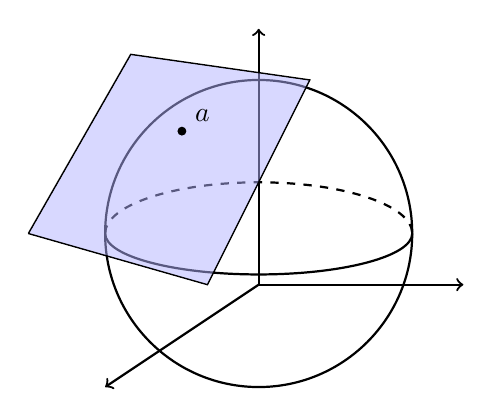
\begin{tikzpicture}[scale=0.65]
	% Esfera
	\draw [thick] (3,0) arc (0:180:3 and -0.8);
	\draw [thick, dashed] (-3,0) arc (180:0:3 and 1);
	\draw [thick] (0,0) circle (3);

	% Ejes R3
	\draw [thick,->] (0,-1) -- (0,4);
	\draw [thick,->] (0,-1) -- (4,-1);
	\draw [thick,->] (0,-1) -- (-3,-3);


	% Rectángulo (Espacio Tangente)
  \draw [fill=blue!30!white,opacity=0.5, line width=0] (-4.5,0) -- (-2.5,3.5) --(1,3.0) -- (-1,-1) -- (-4.5,0);
  \draw [line width=0.5] (-4.5,0) -- (-2.5,3.5) --(1,3.0) -- (-1,-1) -- (-4.5,0);
	\filldraw (-1.5,2) circle (0.075);
	\node at (-1.1,2.3) {$a$};
\end{tikzpicture}

}
    \caption{Representación del espacio \\ tangente a una esfera.}
  \end{figure}
\end{columns}
\end{frame}

\begin{frame}
  Si tenemos un punto $a = (a_1, \dots, a_n) \in \R^n$ y un vector $\begin{bmatrix} v_1 \dots v_n \end{bmatrix}$ podemos parametrizar la recta que pasa por $a$ con dirección $v$ de la siguiente manera:

  \[\gamma(t) = a_1 + tv_1, \dots, a_n + tv_n \]
  \pause
  Teniendo esto en cuenta, y, por nuestros cursos de cálculo sabemos que si $f: \R^n \to \R$ es una función suave definida en un punto $a$ y $v \in T_a(\R^n)$ podemos obtener la derivada direccional de $f$ en $a$ en la dirección de $v$ como:
  \[
    D_v f = \left. \frac{d}{dt}\right|_{t=0} f(\gamma(t)) 
    = \sum_{i=1}^{n} v_i \left. \frac{\partial f}{\partial x_i} \right|_{a}
  \]
\end{frame}

\begin{frame}
  Hay dos propiedades que nos interesan particularmente de la derivada direccional. La derivada direccional es lineal y cumple la regla de Leibniz. Esto quiere decir que si $f$ y $g$ son funciones suaves definida en una vecindad de $a \in \R^n$, $c$ es una constante y $v \in T_{a}(\R^n)$, entonces:

  \begin{itemize}
    \item $D_v(f+g) = D_v(f) + D_v(g)$
    \item $D_v(cf) = cD_v(f)$
    \item $D_v(fg) = f(a)D_v(g) + g(a)D_v(f)$ 
  \end{itemize}
\end{frame}

\begin{frame}
  Basándonos en las propiedades anteriores de las derivaciones es que se darán las siguientes definiciones.
  \begin{definition}[Derivación en un punto]
    Si $a$ es un punto en $\R^n$ y $\omega: C^{\infty}(\R^{n}) \to \R$ es un funcional lineal, diremos que $\omega$ es una \textbf{derivación} en $a$ si cumple la regla de Leibniz. Esto es, si $f$ y $g$ son funciones suaves definidas en una vecindad de $a$ y $c$ es una constante, entonces:
    \begin{itemize}
      \item $\omega(cf) = c \omega(f)$
      \item $\omega(f+g) = \omega(f) + \omega(g)$
      \item $\omega(fg) = f(a)\omega(g) + g(a)\omega(f)$
    \end{itemize}
  \end{definition}

\end{frame}

\begin{frame}
  El conjunto de todas las derivaciones en $a$, el cual denotamos por $\mathcal{D}_a(\R^n)$ es, curiosamente, un espacio vectorial bajo las operaciones:
  \begin{align*}
    (\omega_1 + \omega_2)(f) &= \omega_1(f) + \omega_2(f)\\
    (c\omega)(f) &= c(\omega(f))
  \end{align*} \pause

  Y quizá todavía más curioso es el siguiente teorema:
\end{frame}

\begin{frame}
\begin{theorem}
  Los espacios $T_a(\R^n) \to \mathcal{D}_a(\R^n)$ son isomorfos y el isomorfismo de espacios vectoriales está dado por:
\begin{align*}
  \phi: T_a(\R^n) &\to \mathcal{D}_a(\R^n)\\
  v &\mapsto D_v = \sum_{i=1}^n v_i \left. \frac{\partial}{\partial x_i} \right|_{a}
\end{align*}
\end{theorem}\pause

  Dos consecuencias de este teorema es que el espacio de derivaciones en un punto $a$, $\mathcal{D}_a(\R^n)$ es isomorfo a $\R^n$ y que para cada $a \in \R^n$, las $n$ derivadas parciales:
  \[
    \left. \frac{\partial}{\partial x_1} \right|_a,
    \dots,
    \left. \frac{\partial}{\partial x_n} \right|_a
  \]
  forman una base para el espacio tangente $T_a(\R^n)$
\end{frame}

\begin{frame}
\begin{definition}[Derivación en un punto de una variedad]
  Sea $M$ una variedad suave y sea $p \in M$ un punto. Diremos que en mapa $\omega: C^{\infty}(M) \to \R$ es una \textbf{derivación} en $p$ si es lineal y además cumple la regla de Leibniz.

  Llamaremos al conjunto de todas las derivaciones en un punto de una variedad el \textbf{espacio tangente} a la variedad en ese punto, y denotaremos al conjunto por $T_p(M)$.
\end{definition}\pause

  El espacio tangente $T_p(M)$ también es un espacio vectorial bajo operaciones idénticas a las vistas anteriormente.
\end{frame}

\begin{frame}
  Ahora quisiéramos estudiar como es que los mapas suaves entre variedades afectan a los vectores del espacio tangente.

  \begin{definition}[Diferencial de un mapa]
    Si $M$ y $N$ son variedades suaves y $F: M \to N$ es un mapa suave, entonces para cada punto $p \in M$ el mapa $F$ induce un mapeo lineal entre $T_p(M)$ y $T_{F(p)}(N)$, denotado $dF_p: T_p(M) \to T_{F(p)}(N)$, a este mapa le llamamos el \textbf{diferencial de F en p}.

    El mapa $dF_p$ está dado por: Dada un vector tangente $\omega \in T_p(M)$, $dF_p$ será la derivación en el punto $F(p) \in N$ que actúa sobre funciones suaves $f: N \to \R$ del siguiente modo:
    \[
      dF_p(\omega)(f) = \omega(f \circ F)
    \]
  \end{definition}
\end{frame}

\begin{frame}
  \begin{figure}
    \centering
    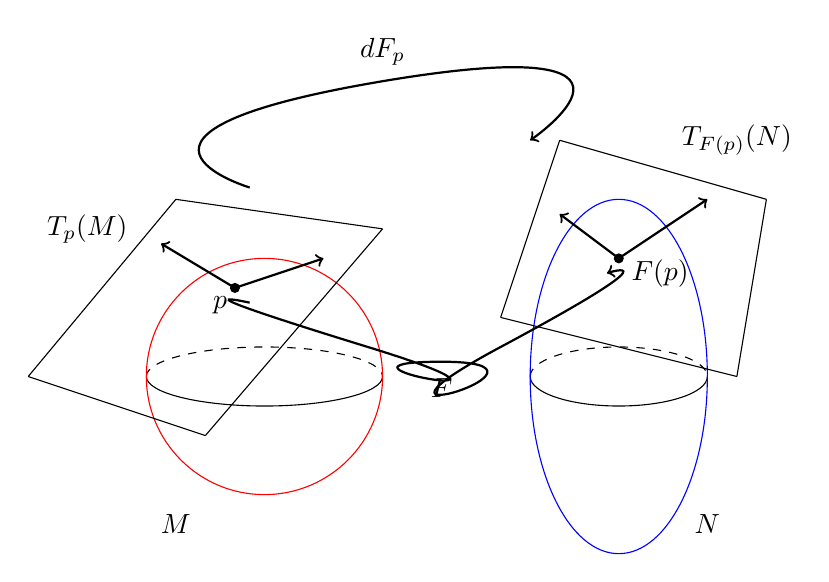
\begin{tikzpicture}[scale=0.75]
  % Esfera
  \draw (-4,0) arc (0:180:2 and -0.5);
  \draw [dashed] (-8,0) arc (180:0:2 and 0.5);
  \draw [red] (-6,0) circle (2);
  \node at (-7.5,-2.5) {$M$};
  \node at (-6.75,1.2) {$p$};
  \node at (-9,2.5) {$T_p(M)$};

  % Rectángulo (Espacio Tangente a Esfera)
  \filldraw (-6.5,1.5) circle (0.075);
  \draw[thick,->] (-6.5,1.5) -- (-5,2);
  \draw[thick,->] (-6.5,1.5) -- (-7.75,2.25);
  \draw  (-7.5,3) -- (-4,2.5);
  \draw  (-4,2.5) -- (-7,-1);
  \draw  (-7,-1) -- (-10,0);
  \draw  (-10,0) -- (-7.5,3);

  % Elipsoide
  \draw (1.5,0) arc (0:180:1.5 and -0.5);
  \draw [dashed] (-1.5,0) arc (180:0:1.5 and 0.5);
  \draw [blue] (0,0) ellipse (1.5 and 3);
  \node at (1.5,-2.5) {$N$};
  \node at (0.7,1.75) {$F(p)$};
  \node at (2,4) {$T_{F(p)}(N)$};

  % Rectángulo (Espacio Tangente a Elipsoide)
  \filldraw (0,2) circle (0.075);
  \draw[thick,->] (0,2) -- (1.5,3);
  \draw[thick,->] (0,2) -- (-1,2.75);
  \draw (-2,1) -- (2,0);
  \draw (2,0) -- (2.5,3);
  \draw (2.5,3) -- (-1,4);
  \draw (-1,4) -- (-2,1);

  % Flechas
  \draw[thick, ->] plot [smooth,tension=4] coordinates {(-6.25,1.25) (-4.25,0.5) (-3,0.25) (-2,0.5) (-0.20,1.75)};
  \node at (-3,-0.20) {$F$};
  \draw[thick, ->] plot [smooth,tension=4] coordinates {(-6.25,3.2) (-4,5) (-1.5,4)};
  \node at (-4,5.5) {$dF_p$};

\end{tikzpicture}

    \caption{Representación del diferencial de un mapa}
  \end{figure}
\end{frame}

\begin{frame}
  Los espacios tangentes son muy útiles, sin embargo, para nuestros fines será necesario ser capaces de considerar más de un espacio tangente a la vez, esto se puede hacer considerando el fibrado tangente.
  
\begin{definition}[Fibrado Tangente]
  Dada una variedad suave $M$, definimos el \textbf{fibrado tangente de $M$}, el cual denotaremos por $TM$, como la unión disjunta de todos los espacios tangentes a $M$:
\[ TM = \bigsqcup_{p \in M} T_p(M) = \bigcup_{p \in M} \{p\} \times T_p(M) \]
\end{definition}
\end{frame}

\begin{frame}
  \centering
  \begin{figure}
  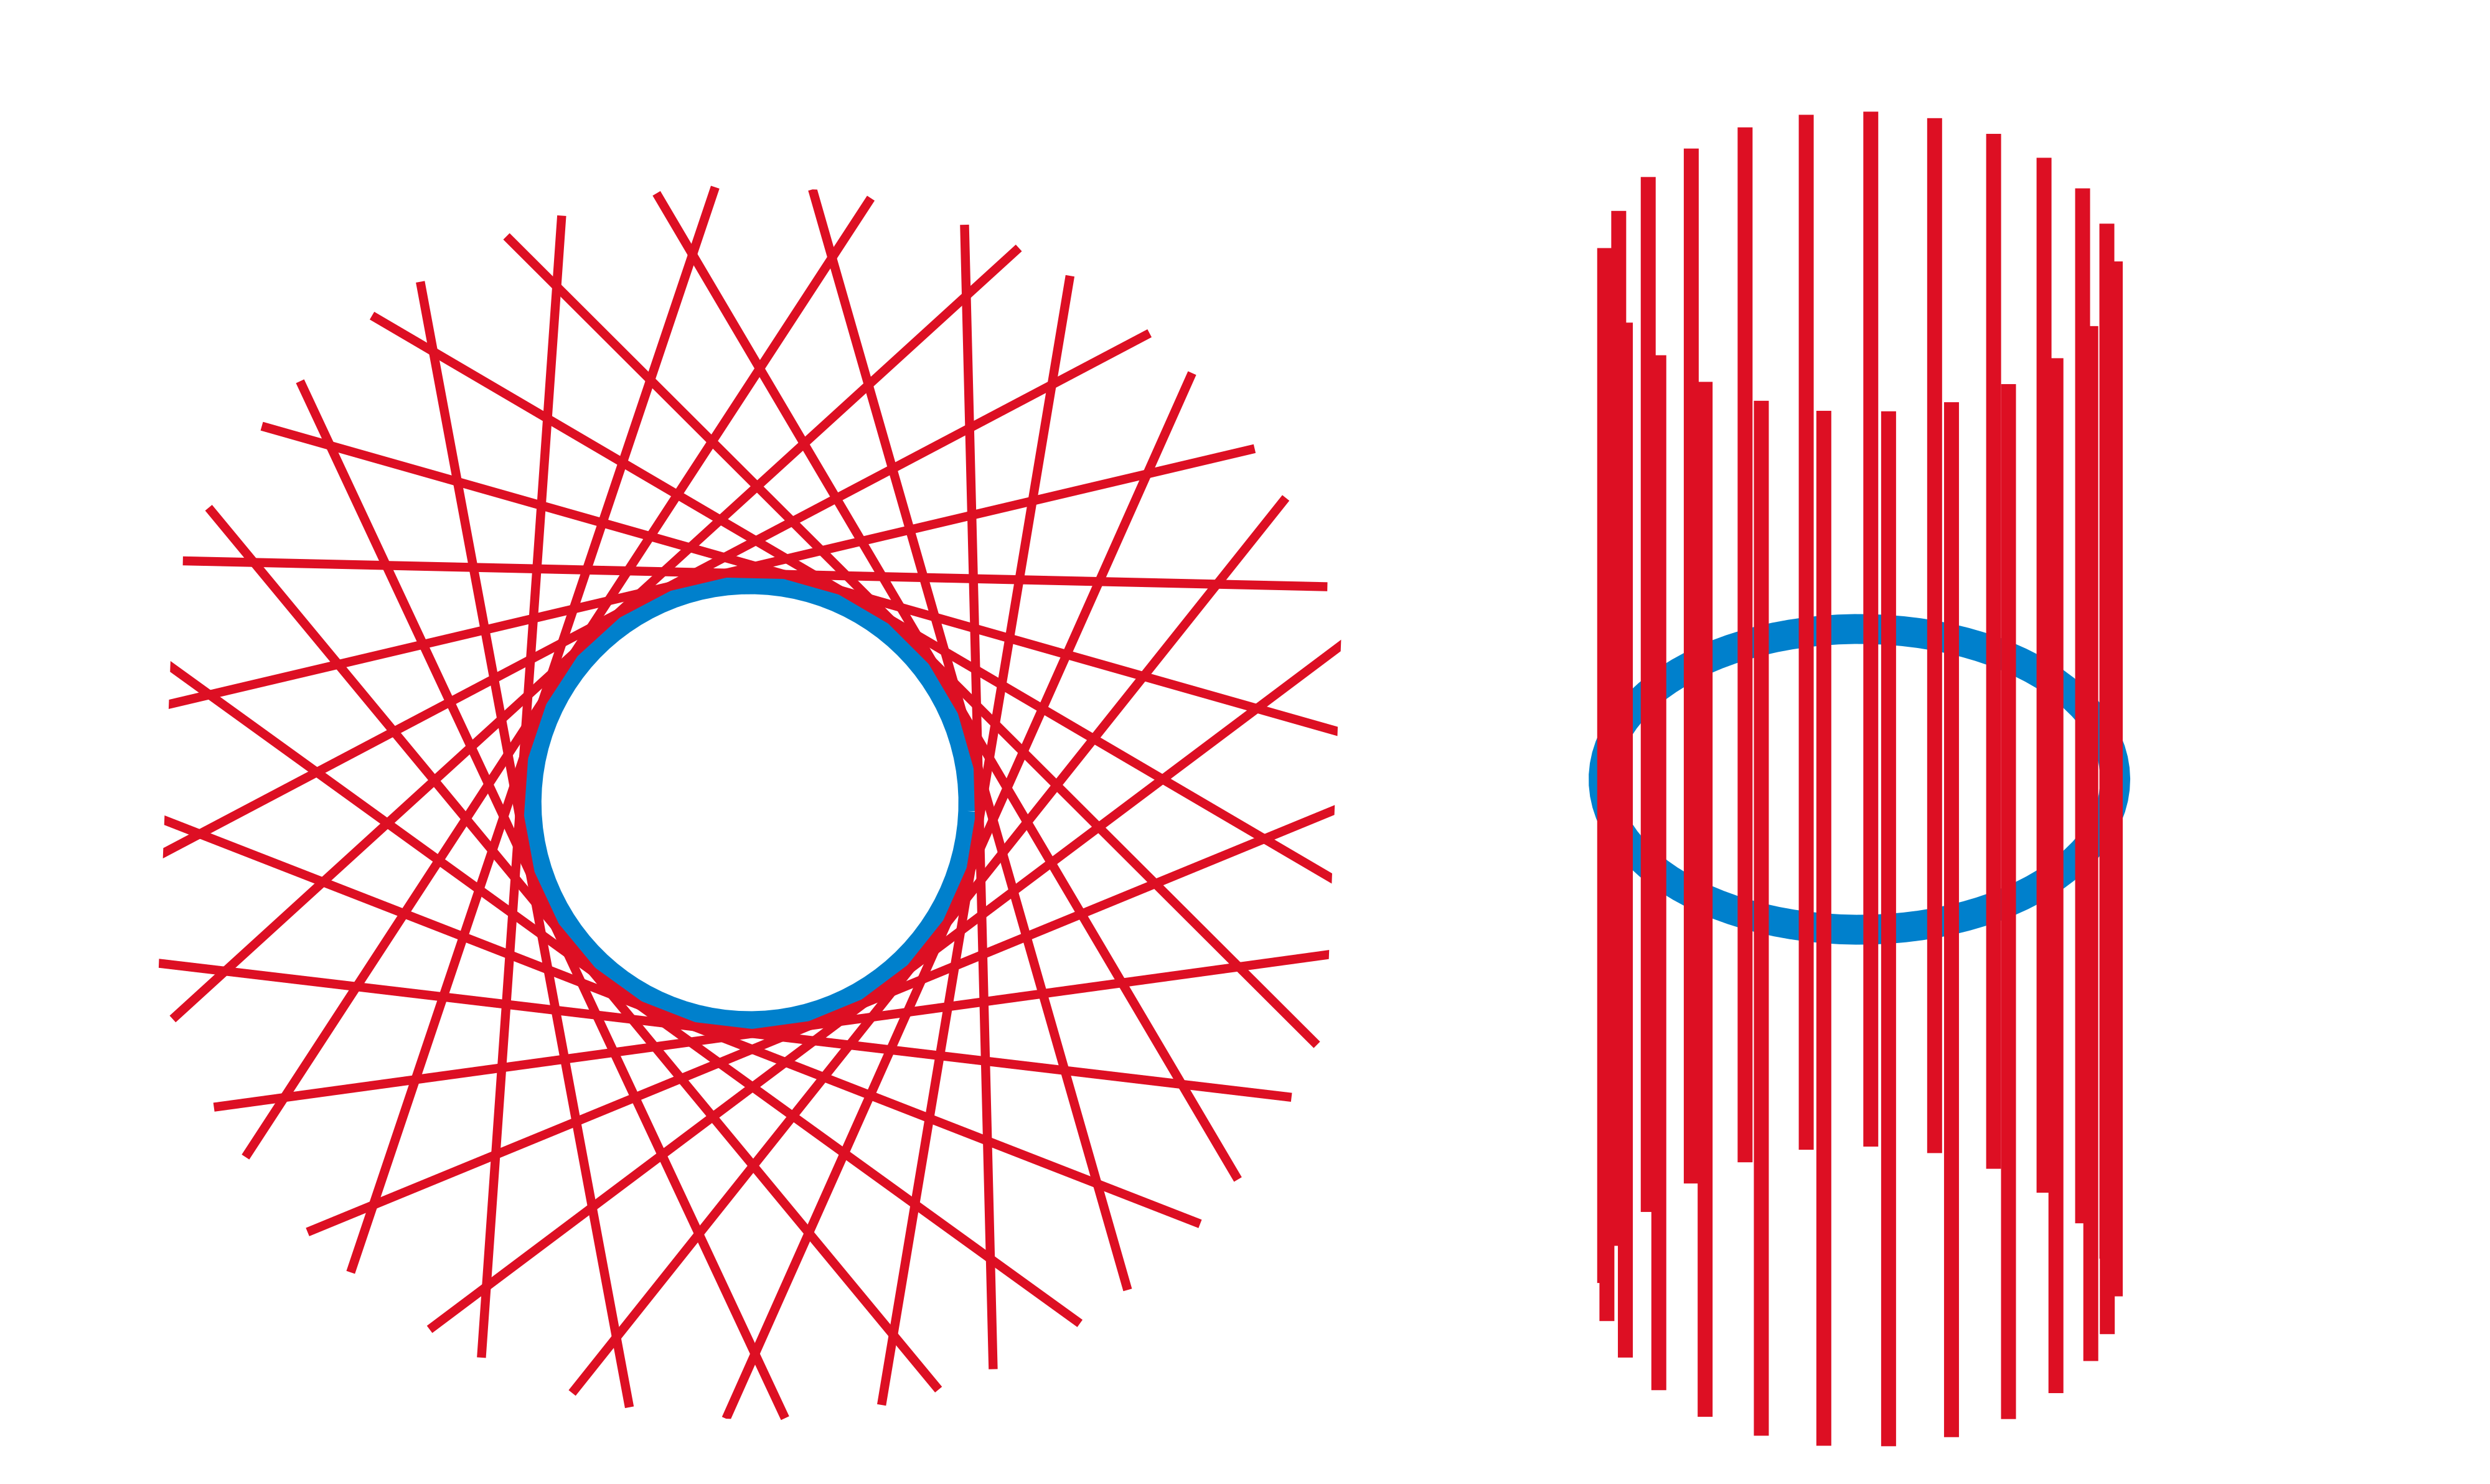
\includegraphics[width=0.8\textwidth]{./Figuras/TangentBundle.png}
    \caption{Espacios Tangentes y Fibrado Tangente de $\S^{1}$.}
  \end{figure}
\end{frame}

\begin{frame}
  \begin{theorem}
    Sea $M^n$ una variedad suave, el fibrado tangente $TM$ tiene una topología natural y una estructura suave que vuelven a $TM$ una variedad suave $2n-$dimensional de tal modo que la proyección $\pi: TM \to M$ es suave con respecto a dicha estructura suave.
  \end{theorem}
\end{frame}


